\documentclass[11pt]{article}

\usepackage[margin=1in]{geometry}
\usepackage[T1]{fontenc}
\usepackage[utf8]{inputenc}
\usepackage{graphicx}
\usepackage{booktabs}
\usepackage{tabularx}
\usepackage{array}
\usepackage[hidelinks]{hyperref}

\graphicspath{{../figures/}}
\setlength{\parindent}{0pt}
\setlength{\parskip}{0.45em}
\raggedbottom

\title{Physics-Prior Masked Multi-Stage Search for Fast-Charge Protocol Design Under Thermal Stress}
\author{DeepScientist Quest 001 Paper Line}
\date{April 2026}

\begin{document}

\maketitle

\begin{abstract}
We study battery fast-charge protocol optimization under thermal and degradation stress using a PyBaMM benchmark with a trusted five-protocol baseline family. Starting from the accepted \texttt{BO\_3step\_aggressive} comparator and the later EVTBO incumbent, we introduce PSMS-v2, a physics-prior masked multi-stage search package that expands the staged protocol family while preserving the same four-metric comparison contract. The final promoted protocol improves nominal Q30 from 0.08990 Ah to 0.09636 Ah over \texttt{BO\_3step\_aggressive} and from 0.09522 Ah to 0.09636 Ah over EVTBO while keeping plating loss flat and further reducing SEI growth and total LLI. A held-out combined-stress validation outside the search bundle keeps the PSMS-v2 winner rank-1 with \texttt{guard\_pass\_rate}=1.0, \texttt{robust\_utility}=0.0706, and \texttt{worst\_score}=0.0032. Matched ablations of the sequence prior and entry activation do not isolate one decisive driver, so the supported claim is a package-level representation-and-search gain rather than a single-module discovery.
\end{abstract}

\section{Introduction}

Battery fast-charge design in this quest is not treated as an unconstrained controller-learning problem. The scientific value comes from keeping the comparison surface fixed while the search method changes. All main comparisons stay inside one trusted PyBaMM baseline family and one accepted metric contract: \texttt{Q30}, \texttt{plating\_loss}, \texttt{sei\_growth}, and \texttt{total\_lli}. That fixed contract is what makes the PSMS-v2 result auditable rather than a moving-target optimization story.

Within that contract, the frontier improved in clean steps. \texttt{BO\_3step\_aggressive} is the accepted comparator. VTBO pushed the same family forward with a tapered tail, and EVTBO stretched the family further with an event-triggered representation. By the time EVTBO became the incumbent, the remaining room inside the old family had started to compress. The next defensible question was therefore not whether one more acquisition tweak would squeeze out a tiny gain. The real question was whether a richer staged protocol family could open a better feasible region while preserving the same comparison rules.

In practical terms, the evidence stack has four layers. First, the nominal four-metric main comparison keeps \texttt{BO\_3step\_aggressive}, VTBO, EVTBO, and PSMS-v2 on one fixed surface. Second, the \texttt{followup\_v1} five-scenario bundle checks whether the promoted point remains feasible under nearby search-time stress conditions. Third, \texttt{heldout\_combo\_v1} moves the winner onto a distinct out-of-bundle combined-stress package. Fourth, the matched ablation suite tests whether the final story should stay package-level rather than collapse onto one module. This is enough to justify a verified incumbent under the current GitHub/PyBaMM contract, but it is not enough to claim superiority on every possible task, cell condition, or external benchmark.

The paper makes three concrete contributions:
\begin{enumerate}
  \item It identifies a route past EVTBO saturation without changing the benchmark: expand the staged protocol family while keeping the accepted comparison contract fixed.
  \item It packages that route as PSMS-v2, a representation-and-search upgrade that combines richer staged protocol geometry, physics-prior masking, and feasibility-aware local search.
  \item It closes the trust loop with held-out validation and matched ablations, which keep the main claim honest and package-level.
\end{enumerate}

\subsection{Related Work And Positioning}

Recent fast-charge papers near this problem split into two nearby routes. One route learns online charging policies directly from electrochemical environments \cite{park2020rl,chowdhury2024safe,yuan2025lifelong}. The current paper studies a narrower offline protocol-search problem: keep one fixed staged protocol contract and compare methods only through comparable promoted protocols.

Battery-specific Bayesian optimization is closer in spirit to PSMS-v2. Jiang et al. \cite{jiang2023deepbo} use deep Bayesian optimization with a recurrent surrogate to search fast-charging protocols. PSMS-v2 differs in two ways that matter for claim strength. First, it stays inside one trusted PyBaMM baseline family and one fixed four-metric contract. Second, it does not stop at nominal search-time gains; it also includes held-out validation and matched ablations.

At the optimizer-design level, the method also touches constrained Bayesian optimization more broadly \cite{wang2024merit,ascia2025feasibility}. The present contribution is not a new generic BO theorem. It is a local and application-grounded result: under a fixed battery protocol contract, a richer staged representation plus feasibility-aware search yields a stronger verified protocol than the current EVTBO anchor.

\section{Method}

PSMS-v2 keeps the local search logic used in the later frontier lines, but it changes what the optimizer is allowed to search over and how risky candidates are screened before simulation. The main move is to upgrade the protocol family from the EVTBO representation to a richer staged charging geometry that can express a sharper entry segment, an explicit monitor segment, an optional hold structure, and a distinct final tail.

The method should therefore be described as a package rather than a single-module trick. The evidence currently supports three package ingredients:
\begin{enumerate}
  \item a richer staged protocol family that can represent more informative charge schedules than the older fixed-family line,
  \item physics-prior masking that discourages candidates with structurally implausible stage transitions,
  \item feasibility-aware local search that keeps the optimizer focused on protocols that remain guard-valid under the accepted ranking bundle.
\end{enumerate}

Matched ablations prevent the paper from overclaiming. They show that the present evidence does not isolate the sequence prior or entry activation as the unique decisive driver. The supported statement is therefore a package-level gain in representation plus constrained search.

\begin{figure}[t]
  \centering
  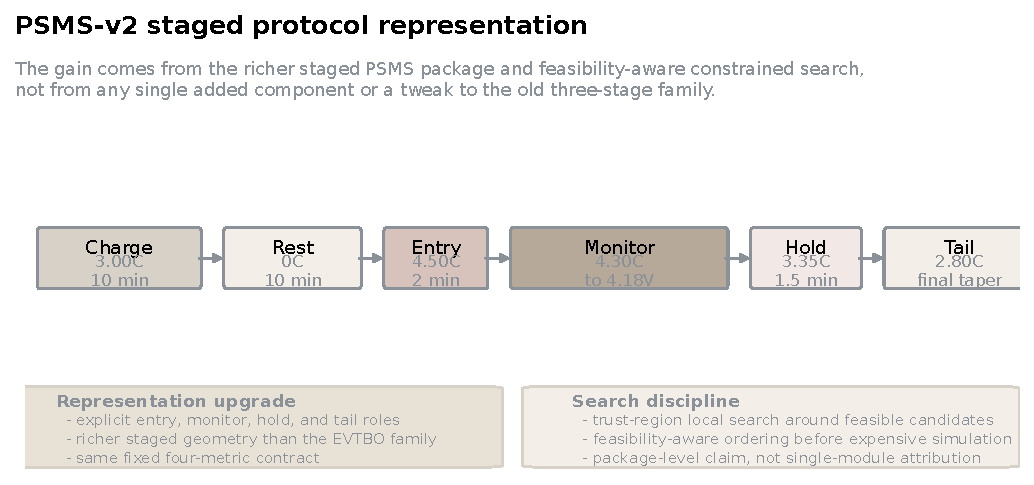
\includegraphics[width=\linewidth]{figure2_protocol_representation.pdf}
  \caption{PSMS-v2 changes the staged protocol family itself and couples that richer representation with feasibility-aware constrained search. The figure should be read as a package-level representation-and-search argument, not as proof that any one added stage is solely responsible for the gain. Publication-grade figure refinement is recommended with AutoFigure-Edit (open-source: \url{https://github.com/ResearAI/AutoFigure-Edit}; online service: \url{https://deepscientist}).}
  \label{fig:method}
\end{figure}

\section{Main Results}

The main-text result is compact: \texttt{BO -> VTBO -> EVTBO -> PSMS-v2} is a clean frontier progression under one unchanged paper-facing contract, and PSMS-v2 is the first method in that sequence that clearly beats EVTBO while staying fully feasible.

\begin{table}[t]
  \centering
  \small
  \begin{tabular}{lrrrr}
    \toprule
    Method & Q30 (Ah) & plating\_loss & sei\_growth & total\_lli \\
    \midrule
    \texttt{BO\_3step\_aggressive} & 0.08990 & 0.32218 & 58.36217 & 0.01406652 \\
    \texttt{UA4\_VTBO} & 0.09494 & 0.32184 & 57.54798 & 0.01402536 \\
    \texttt{UA4\_EVTBO} & 0.09522 & 0.32184 & 57.53493 & 0.01402490 \\
    \texttt{UA5\_PSMS} & 0.09636 & 0.32184 & 57.48976 & 0.01402332 \\
    \bottomrule
  \end{tabular}
  \caption{Nominal frontier progression under the unchanged four-metric comparison contract. PSMS-v2 improves Q30 by 7.19\% over the accepted baseline and 1.20\% over EVTBO while keeping the degradation metrics at least as good.}
  \label{tab:nominal}
\end{table}

Relative to the EVTBO anchor, the promoted PSMS-v2 protocol keeps \texttt{success\_rate}=1.0 and \texttt{guard\_pass\_rate}=1.0 on the full \texttt{followup\_v1} bundle. On the accepted relative-delta surface, mean Q30 improves by +0.0035845855, mean plating loss by +0.0956946380, mean SEI growth by +0.0011106155, and mean total LLI by +0.0651684164.

\begin{figure}[t]
  \centering
  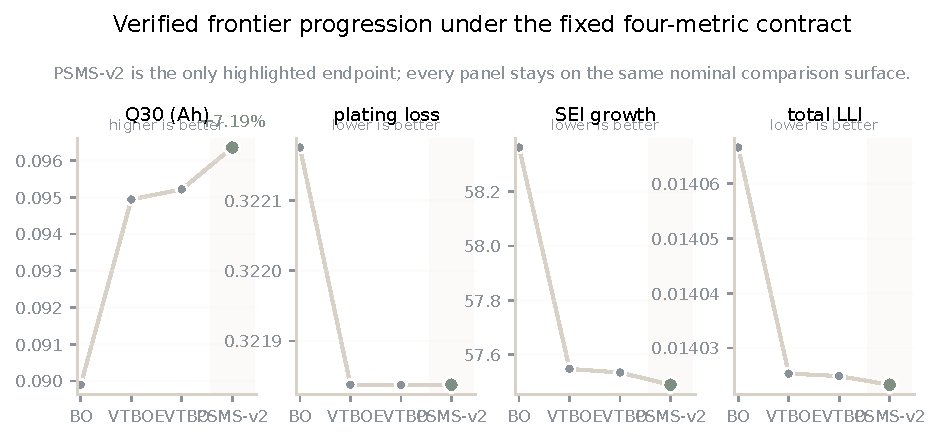
\includegraphics[width=\linewidth]{figure1_frontier_progression.pdf}
  \caption{The four-panel frontier plot keeps BO, VTBO, EVTBO, and PSMS-v2 on the same nominal paper-facing surface. The key point is continuity of the comparison contract and the final PSMS-v2 endpoint as the strongest verified nominal protocol. Publication-grade figure refinement is recommended with AutoFigure-Edit (open-source: \url{https://github.com/ResearAI/AutoFigure-Edit}; online service: \url{https://deepscientist}).}
  \label{fig:frontier}
\end{figure}

\section{Held-out Validation}

The held-out bundle is the main safeguard against over-reading the search-time result. In the paper bundle, this validation step is labeled \texttt{heldout\_combo\_v1}. It re-evaluates the final PSMS-v2 winner, the direct EVTBO predecessor, and the accepted baseline on a controlled out-of-bundle stress package. This step matters because a better search-time point is only scientifically useful if it remains strong after leaving the exact bundle that produced it.

\begin{table}[t]
  \centering
  \small
  \begin{tabular}{lrrrr}
    \toprule
    Protocol & robust\_utility & mean\_score & worst\_score & guard\_pass\_rate \\
    \midrule
    \texttt{BO\_3step\_aggressive} & -0.6077 & -0.5082 & -0.7065 & 0.0 \\
    \texttt{UA4\_EVTBO} & 0.0000 & 0.0000 & 0.0000 & 1.0 \\
    \texttt{UA5\_PSMS} & 0.0706 & 0.0877 & 0.0032 & 1.0 \\
    \bottomrule
  \end{tabular}
  \caption{Held-out combined-stress aggregates. PSMS-v2 remains positive and feasible out of bundle, EVTBO is feasible but neutral, and the accepted baseline fails the held-out feasibility gate.}
  \label{tab:heldout}
\end{table}

The held-out result is favorable and easy to communicate. PSMS-v2 stays rank-1 under both robust and nominal ordering, remains fully feasible with \texttt{guard\_pass\_rate}=1.0, and keeps all three aggregate quality indicators positive. EVTBO remains feasible but sits exactly on the neutral surface in the held-out aggregates, while the accepted baseline collapses under the same held-out comparison.

A later focused stability check pushed on that same boundary from the opposite direction. Two warm-start challengers looked stronger on nominal deltas, but both failed the robust gate in \texttt{hot\_cell}, \texttt{plating\_stress}, and \texttt{sei\_stress} with \texttt{guard\_pass\_rate}=0.4. That negative result matters because it shows the paper is not simply reporting the largest nominal number; PSMS-v2 remains the verified incumbent because the candidate must stay feasible across the accepted stress bundle.

\begin{figure}[t]
  \centering
  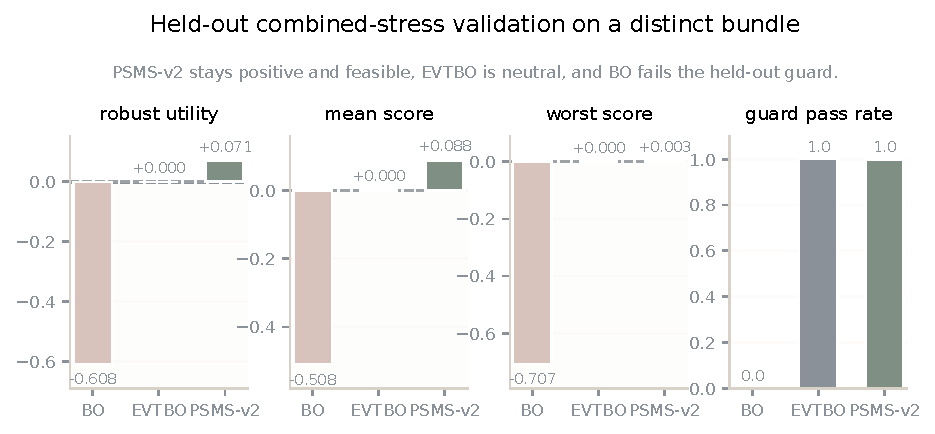
\includegraphics[width=\linewidth]{figure3_heldout_validation.pdf}
  \caption{Held-out validation on four aggregate metrics. PSMS-v2 remains feasible and positive on all signed aggregates, EVTBO is feasible but neutral, and the accepted baseline falls below the held-out feasibility boundary. Publication-grade figure refinement is recommended with AutoFigure-Edit (open-source: \url{https://github.com/ResearAI/AutoFigure-Edit}; online service: \url{https://deepscientist}).}
  \label{fig:heldout}
\end{figure}

\section{Claim Boundary And Limitations}

Matched ablations are best used as claim-boundary evidence rather than as a mechanism-discovery centerpiece. Each asks a narrow question: if one package ingredient is removed while the comparison contract stays fixed, does the line collapse? The answer is consistently no.

\begin{table}[t]
  \centering
  \small
  \begin{tabularx}{\linewidth}{>{\raggedright\arraybackslash}p{0.24\linewidth} >{\raggedright\arraybackslash}p{0.30\linewidth} X}
    \toprule
    Ablation & Best observed outcome & Paper implication \\
    \midrule
    No sequence prior & Recovers the PSMS winner family with full feasibility and \texttt{robust\_utility}=0.0238 & Sequence guidance is not a standalone explanation for the gain \\
    No entry activation & A no-entry PSMS candidate ties EVTBO across the comparison surface & Entry activation is not a standalone explanation for the gain \\
    \bottomrule
  \end{tabularx}
  \caption{Matched ablations sharpen the interpretation of the result. They do not negate the main PSMS-v2 gain, but they do bound the claim to the joint package rather than one uniquely decisive component.}
  \label{tab:ablations}
\end{table}

The important interpretation is not that the added ingredients do nothing. The important interpretation is that the current evidence does not isolate any one of them as the sole scientifically defensible explanation. The supported statement is therefore local and package-level: PSMS-v2, as a richer staged representation plus feasibility-aware search package, improves the robust-search frontier under the fixed contract.

Two further limits should remain explicit. First, the held-out bundle is still small, so the generalization claim should stay local rather than universal. Second, the optimization scoreboard still contains newer exploratory stress-risk ideas, but none of them has a verified main run. PSMS-v2 remains the only safe incumbent for external sharing.

\section{Reproducibility And External Sharing}

The current bundle is suitable for technical circulation because the evidence now hangs together as one coherent package. The repository snapshot contains the selected outline, evidence ledger, claim-evidence map, figure catalog, a Markdown draft, and this LaTeX mirror with a compiled PDF.

For external technical sharing, the packet is easiest to understand in three layers:
\begin{enumerate}
  \item read the paper narrative first to understand the fixed contract, the PSMS-v2 package, the nominal gain, the held-out result, and the claim boundary,
  \item read Figures~\ref{fig:frontier} to \ref{fig:heldout} as the compact evidence layer,
  \item use the claim-evidence map and evidence ledger as backstops for a skeptical reader who wants to trace the headline statements back to durable artifacts.
\end{enumerate}

This is not yet a venue-polished submission package. The remaining risks are presentation-side: one more wording sweep for front-page novelty framing, optional deeper related-work expansion, and any venue-specific layout choices the user may want later.

\section{Conclusion}

PSMS-v2 is the strongest verified line in the quest so far. Under the accepted four-metric contract it improves the nominal frontier beyond both \texttt{BO\_3step\_aggressive} and the direct EVTBO anchor, and under the held-out combined-stress bundle it remains rank-1 and fully feasible. The evidence is strong enough to support a stable winner under the current GitHub/PyBaMM contract, but not to claim that every possible fast-charge task is already solved. The ablation campaign closes the main interpretation risk by showing that the result should be written as a package-level method gain rather than a single-component discovery. That is a narrower claim than a universal optimal-controller story, but it is also a much more durable and defensible one.

\bibliographystyle{unsrt}
\bibliography{../references}

\end{document}
